% status: 85
% chapter: TBD
\title{Simple Linear Regression API with Flask}



\author{Janaki Mudvari Khatiwada}
\affiliation{%
  \institution{Indiana University}  
  \city{Bloomington} 
  \state{IN} 
  \postcode{47408}
  \country{USA}}
\email{janu.khatiwada@gmail.com}


% The default list of authors is too long for headers}
\renewcommand{\shortauthors}{J. M. Khatiwada}



\begin{abstract}
  Python's flask application requires minimal application for application
  development. Flask make use of backend data as a resource to support an
  application running on the server. This project discusses development
  and deployment of REST api with python flask. This flask api gets predict
  info based on regression model created from car data set. Once flask app runs 
  successfully, it is then deployed to Heroku, a platform as a service 
  cloud platform. For the purpose car data set from UCI machine learning
  data repository is being used. Before this a regression model for the
  data has to be build to make sure that this model best describes the 
  relationship between variables, in this case engine size and highway
  miles per gallon. Based on this model new data set can be tested to make 
  to make prediction. Then regression results is used as the endpoint 
  in flask api.
   
\end{abstract}

\keywords{e516, hid-sp18-415, Flask, Cloud Computing, Regression Model }


\maketitle`

\section{Introduction}
  Flask api framework requires mimimal framework for restful web services.
  Rest services is an architectural style web services which use HTTP protocol
  to establish communication between client and server for each service request.
  Being lightweight and scalable, flask is chosen as a good option for 
  developing to develop RESTful apis. The main purpose of this paper is
  to create a regression model for car data set. The model is intended to
  predict highway miles per gallon based on engine size of the vechicle.
  Simple linear regression is run using scikit-learn. This model is going
  to be the resource in flask api. Using GET and POST methods to call
  endpoints. GET method fetch resource info while POST method creates
  a new resource. Resource for API can be in different format but json format
  is easy understand and flask has in-built support for the format. So 
  our resource will be our json object and stored in key--value pair.
  
  Once flask api is succesfully run in localhost, the application is
  then deployed to heroku which is an open source platform as a 
  service cloud platform. This also has a minimal deployment needs.
  They are open an account in heroku.com, then download heroku
  command line interface(CLI). Then run heroku login from CLI and
  and create an app. This is discussed in more detail under section
  methods.
  
 
 
\section{Simple Linear Regression}
  Just to provide a brief overview of why simple linear regression is
  chosen for the project, a brief introduction about it would be
  appropriate .Linear Regression is a statistical data analysis tool
  which describes the effect of one variable also called independent
  variable on dependent variables. In case of simple linear regression
  there is only one dependent variable with one independent variable
  just like in multiple regression. Our purpose of running this project
  is to create a line of best fit model build a model that can be used
  for prediction. In this case prediction of mpg based on engine size
  of the vehicle. The line of best fit is described by the
  formula \[y = a + bx\] where a is coefficient or y intercept and b is
  slope for the line. In this case formula for prediction model or
  regression is given below, where hwy\_mpg is y variable and
  engine\_size is x variable.
  \[hwy\_mpg = yintercept + slope.enginesize\] 
\section{Methods}
  Data selection, cleaning and preprocessing, building a local
  environment, building a linear regression model using SciKit--learn,
  designing a REST api with Flask and running locally and deploying
  it into heroku are the main
  processes of this project. They are explained below under each bullet
  points:
\begin{itemize}
    \item Automobile Data Set, \textit{https://archive.ics.uci.edu/ml/
          machine--learning-databases/autos/imports--85.data}, from UCI
          Machine learning data repository is selected. It was created
          in 19 May, 1987 by Jefferey C. Schlimmer \cite{uci-com}. The
          data set is multivariate with 25 attributes. Since the project
          is more focused on designing and deploying a simple linear
          regression api as a demonstration of implementing Flask service,
          only two attributes, `engine size' and `highway miles per gallon'
          are used. Rest of the attributes are dropped. The goal of the
          project is to build a best fit prediction model for highway mpg
          based on engine size. The data set have several missing instances
 as well which are removed as a clean up process. Cleaned data is stored in
 google Dropox as a csv   file so that it can be easily fetched into the
 application. It is located in \textit{https://www.dropbox.com/s/986566hudfytl8h/cardata.csv?dl=0}.
    \item Ubuntu 16.04 is the operating system used for whole project.
  A virtual environment pyenv is created in Ubuntu 16.04 where python 3
 environment is build. Besides, flask, this project requires different python
 packages to fetch and manipulate data and run linear regression and
 then build a flask api. Using pip install package name, packages Flask,
 pandas, numpy, scipy and SciKit--learn are installed. Besides these
 packages, python packages matplotlib and seaborn are installed as they
 are required to create a regression plot and and plot line of best fit. 
    \item Next is building a model from the data set. This is done by
 running python's machine learning application. There are two types of
 machine learning, supervised and unsupervised learning. Supervised
 Machine learning is learning properties of data set (training data set)
 and applying them to the test data set. This machine learning algorithm
 is also called supervised learning. Regression problem in Scikit--learn
 is supervised machine learning. In this case predicting highway mpg for
 the new data set based on engine size is the regression problem.
    
    Regression analysis or building a best fit model for our data set is
   discussed in detail under section Analysis and Algorithm. Now the data
   set is split into two sets one used for defining a regression 
   equation. This equation is going to be the prediction model for data.
   Once regression equation is defined
   that is value for slope and intercept is calculated.   
   Source codes are located in github repository \cite{regression}.
    \item The final process is writing a flask api which can be run to call 
 endpoints using `GET' and `POST' methods. In this project predict is the
 endpoint for POST method and and current details is the endpoint for GET
 method. Then this application is deployed into heroku cloud platform from
 CLI. Before deploying `heroku create app--name' is run to create an app within
 heroku. Then run `git init' to initiate a remote git repository, since app is 
 deployed through git push. In order to deploy to heroku it needs `Procfile'
 with the process it needs to run and requirements.txt or Pipfile that has lists 
 of dependencies needed for the app. Since this api needs to run regression, all
 the needed packages numpy, scipy, pandas and scikit-learn are configured from 
 'heroku config buildpacks'. Then run `git remote', `git add .' to add files,  
 `git commit' and `git push heroku master'.
\end{itemize}    

\section{Analysis and Algorithms}
  The cleaned data set has two attributes \textit{engine size} and
  \textit{highway miles per gallon} and 199 data points. Before developing
   a flask api, a linear regression machine learning model is created using
   scikit-learn. As discussed earlier this is going to be the prediction model
   and one of the endpoints for flask api.

   As it is mentioned above data set is split into two, one is train
   set and other is test set using algorithm train\_set\_split. 
   Train--set data is used to build the regression
   model. In order to train data set, we move label column to its own data frame
   called `train\_labels by pulling  series``hwy\_mpg'' from 
   train--set \cite{regression}. Then `LinearRegression' class is created and fit 
   method is called by \[lin_reg = LinearRegression()\] 
   \[lin_reg.fit(train_set, train_labels)\]. Now we calculate intercept and
  slope our model. These values are used to create model formula
  as discussed in linear regression section above. Then predict function is
  called  by passing series test\_set which returns an array of predicted 
  values \cite{regression}. This model can be checked by calling print function
  for hwy\_mpg\_pred
  and test\_set series and compare values for each series. Another method to
  chesk how significant the model is by calculating the value for r--square 
  which in this case is lin\_reg score by running following algorithm.  
  \[lin\_reg.score(test\_set, test\_set\_full[``hwy_mpg''])\]
  The value of this score ranges between --1 to 1. Scores closer to negative 1
  tells negatively impacted model and that closer to positive one shows positive 
  impact on the model.
  
  After defining the model flask api is developed where just created model will 
  be the resource object. But before this, we should make sure the model do not 
  change when new data points are added. For the purpose we use joblib which can
  handle arrays stored in the models.
  
   
  
\section{Results and Discussion}


  
\section{Conclusion}

Put here an conclusion. Conclusion and abstracts must not have any
citations in the section.


\begin{acks}

  The authors would like to thank Dr.~Gregor~von~Laszewski for his
  support and suggestions to write this paper.

\end{acks}

\begin{figure}[htb]
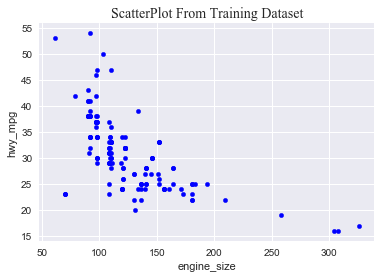
\includegraphics[width=1.0\columnwidth]{images/scatterplot.png}
  \caption{Scatter Plot Engine size and Highway MPG \cite{}}
  \label{scatterplt}
\end{figure}

\begin{figure}[htb]
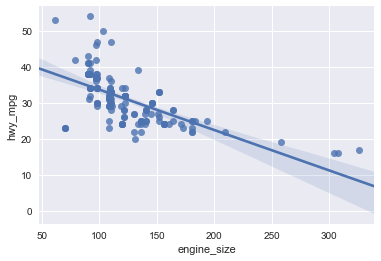
\includegraphics[width=1.0\columnwidth]{images/reg_plot.png}
  \caption{Regresssion Plot Engine size and Highway MPG \cite{}}
  \label{regplt}
\end{figure}

\begin{figure}[htb]
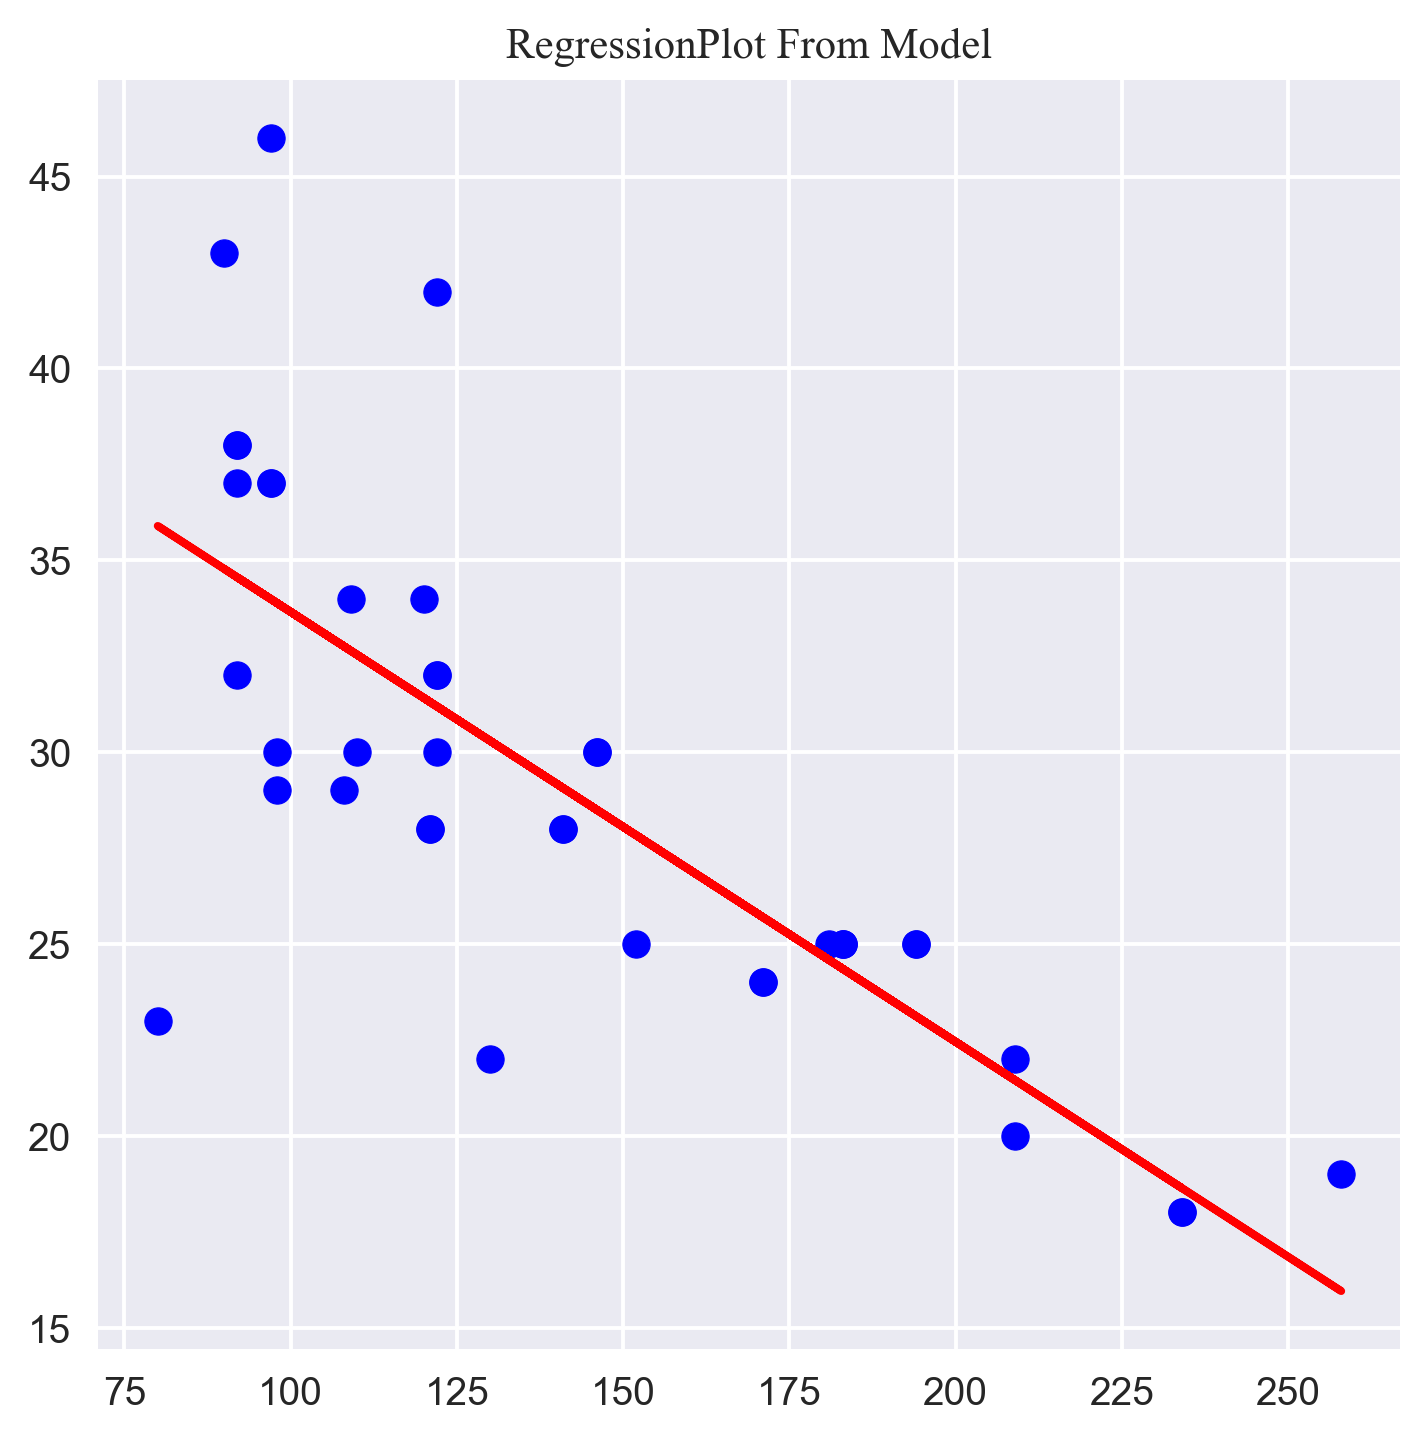
\includegraphics[width=1.0\columnwidth]{images/plot_pred_test_set.png}
  \caption{Prediction Plot Engine size and Highway MPG \cite{}}
  \label{regplt}
\end{figure}

\bibliographystyle{ACM-Reference-Format}
\bibliography{report} 
